\documentclass{my-article}
\usepackage{my-coverpage}
\usepackage{my-codespace}

\usepackage[utf8]{inputenc}
\usepackage[T5]{fontenc}
\usepackage[vietnamese]{babel}

\usepackage{textcomp}
% =========================
% Cover page information
% =========================

\NameUpperUniname{Vietnam National University Ho Chi Minh City}
\NameUniname{Ho Chi Minh City University of Technology}
\NameDeptname{Faculty of Electrical and Electronics Engineering}
\NamePathlogo{./my-chapters/my-images/01_logobachkhoatoi.png}
\NameClass{Digital System Design \\ &  and Verification (EE3213)}
\NameGroup{04}
\NameLesson[\Large]{HOMEWORK REPORT}
\NameTitle[\Huge]{Chương 3 - Thiết kế mạch tổ hợp}
\NameAdvisor{Nguyễn Trung Hiếu}
\NamePlace{Ho Chi Minh}
\NameTime{../../20..}
\NamePathBackground[width=\paperwidth,height=\paperheight]{./my-chapters/my-images/bia.jpg} 
\MemberTableData{
1 & 2213874 & Nguyễn Thanh Tùng & L01 \\ \hline
2 & 2210780 & Nguyễn Đại Đồng & L01 \\ \hline
3 & 2213496 & Nguyễn Quốc Tín & L01 \\ \hline
}

% =========================
% Configuration
% =========================
%--- Header and footer
\fancyhf{}
\fancyhead[L]{\leftmark}
% =========================
% Document
% =========================

\newcommand{\question}[1]{%
	\section*{#1}%
	\addcontentsline{toc}{section}{#1}%
}
\newcommand{\answer}[2]{%
	\subsection*{\textbf{#1}\kern0.2em)~#2}%
	\addcontentsline{toc}{subsection}{#1)}%
}

\newcommand{\finalresult}[1]{%
	\begin{tikzpicture}[baseline=(content.base)]
		\node[draw=red, thick, rounded corners=3pt, inner sep=6pt] (content)
		{\ensuremath{#1}};
	\end{tikzpicture}%
}

\begin{document}
\pagestyle{empty}
\MycoverFinalProject % Cover page
\newpage
\renewcommand{\arraystretch}{1.5} % tăng khoảng cách dòng (row height)
\setlength{\parindent}{1cm}
\onehalfspacing
\setlength{\parskip}{6pt} 
\tableofcontents
\listoffigures
\listoftables
\listoflistings
\newpage
\pagestyle{fancy}
\MycountPages{number}
\fancyhead[R]{GVHD: Nguyễn Trung Hiếu}
\fancyfoot[L]{
\includegraphics[width=.02\linewidth]{./my-chapters/my-images/logo_DEE.png}\text{ Department of Electronics}}

\question{Câu 6}

Thiết kế một bộ sắp xếp song song như hình dưới, mô tả giải thuật sắp xếp 8 mẫu ngõ vào $x_{1}$, $x_{2}$,$\dots, x_{8}$, và cho ngõ ra là $y_{1}$, $y_{2}$, $\dots, y_{8}$ theo thứ tự giảm dần (hoặc tăng dần).

\begin{figure}[H]
	\centering
	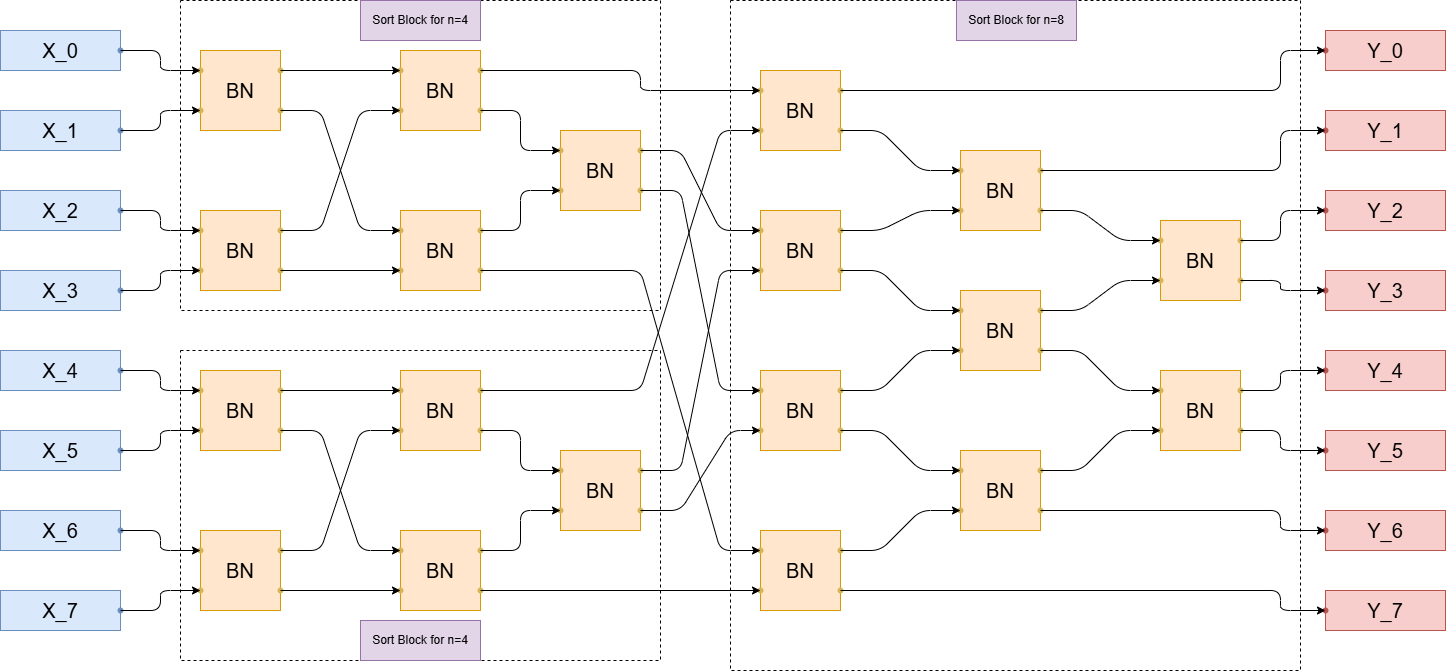
\includegraphics[width=\linewidth]{./my-chapters/my-diagrams/Question6/debai.png}
\end{figure}

Trong đó, mỗi bộ BN (Bitonic Sort) có cấu trúc như hình:

\begin{figure}[H]
	\centering
	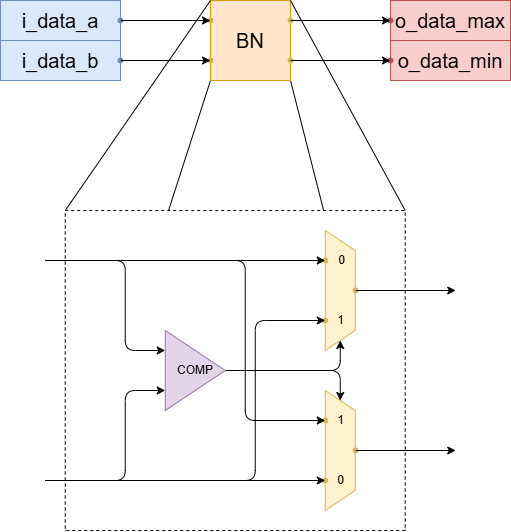
\includegraphics[width=.4z\linewidth]{./my-chapters/my-diagrams/Question6/Swap_and_compare.png}
\end{figure}

Cho các standard cell là: Cổng NOT, các cổng logic 2 ngõ vào, Mux 2-1, Mux 4-1.
\end{document}
